This section gives the full results of the pocket-edit test. Figure~\ref{fig:main} shows the predicted against the measured change on the 19 held-out targets. In this section the geometry network is ResidueSum-Geo, the geometry-free network is ResidueSum and the edit-record network is ResidueSum-Edit.

\subsection{Truncating pocket residues changes docking scores in a structured way}

The cost and the recall reported in the main text say how well a shared-state network reproduces docking scores. DockMut-1 asks what the score of the network follows when the pocket changes, and the docking engine supplies the answer for every ligand. Re-docking the wild-type receptor with different seeds scatters the score of one ligand by \sigmaMed{}~\kcal{} (median over \nTargets{} targets, range \sigmaMin{} to \sigmaMax{}). A measured change is the score of the edited receptor minus the mean of the wild-type replicates, so its noise is \dsigmaMed{}~\kcal{}, and changes beyond twice that value are counted as clear. Independent docking of \vinaEdits{} edits with AutoDock Vina 1.1.2 (the two single and the two multi-residue truncations with the largest measured effect on each of three training targets) reproduces the changes measured with the GPU engine, with $r$ = \vinaR{} over \vinaN{} ligand-edit pairs of \vinaLigPerEdit{} ligands per edit, \vinaWithinR{} within edits and \vinaEditR{} for the edit means (subsection Re-docking protocol and validation of the extended methods). Truncations of shell and far residues serve as a negative control. Their changes have a standard deviation over ligands of \sdNull{}~\kcal{}, close to the replicate noise, and \fracNull{}\% of their ligands change by more than twice that noise. Single contact truncations scatter the changes with a standard deviation of \sdSingle{}~\kcal{} and move \fracSingle{}\% of the ligands beyond twice the noise, and multi-residue contact truncations give \sdMulti{}~\kcal{} and \fracMulti{}\% (Figure~\ref{fig:response}b). Across the \nContactEdits{} contact truncations the standard deviation of the change grows with the number of removed atoms ($r$ = \rNremoved{}) and falls with the distance of the residue from the box center ($r$ = \rDmin{}), and within single truncations the correlations are \rNremovedSingle{} and \rDminSingle{}.

\begin{figure}[!ht]
\centering
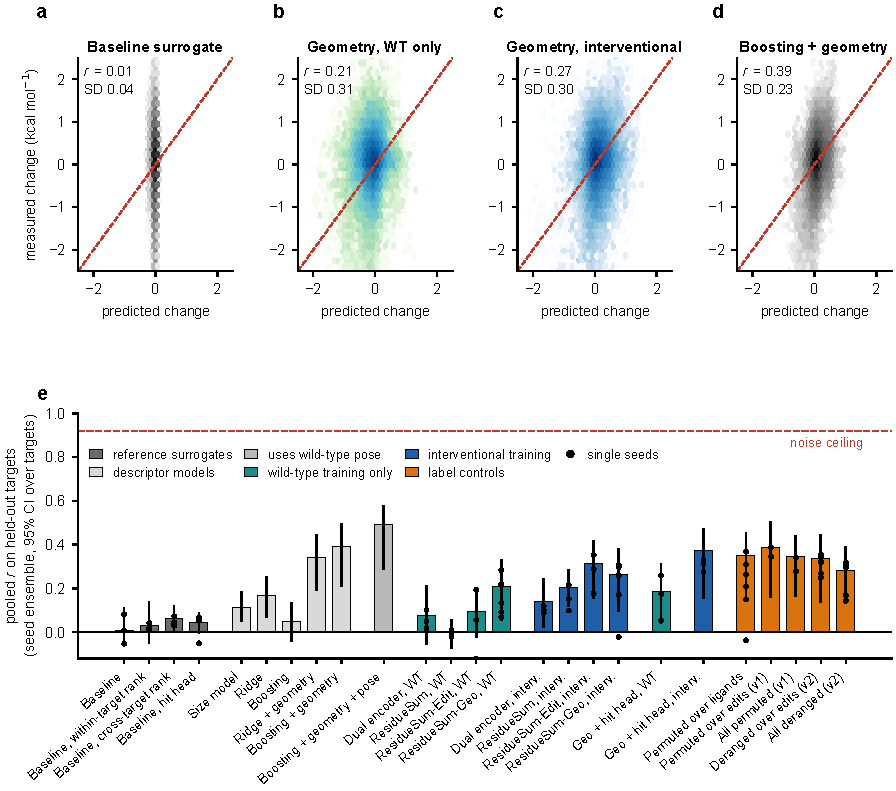
\includegraphics[width=\linewidth]{figures/fig3_main}
\caption{Prediction of measured score changes on the 19 held-out targets. (a--d) Predicted against measured change for the ensemble of the baseline surrogates, the geometry network trained on wild-type scores, the geometry network trained on measured changes and a boosting model on descriptors (hexagonal bins, logarithmic color, dashed line = identity), with the correlation $r$ and the standard deviation of the predicted change in \kcal{}. (e) Pooled correlation of every condition for the seed ensemble (bars, 95\% interval over targets) and for single seeds (dots). The dashed line marks the noise ceiling set by the wild-type replicates. v1 is the first implementation of a permutation control and v2 its correction.}
\label{fig:main}
\end{figure}

\begin{figure}[!ht]
\centering
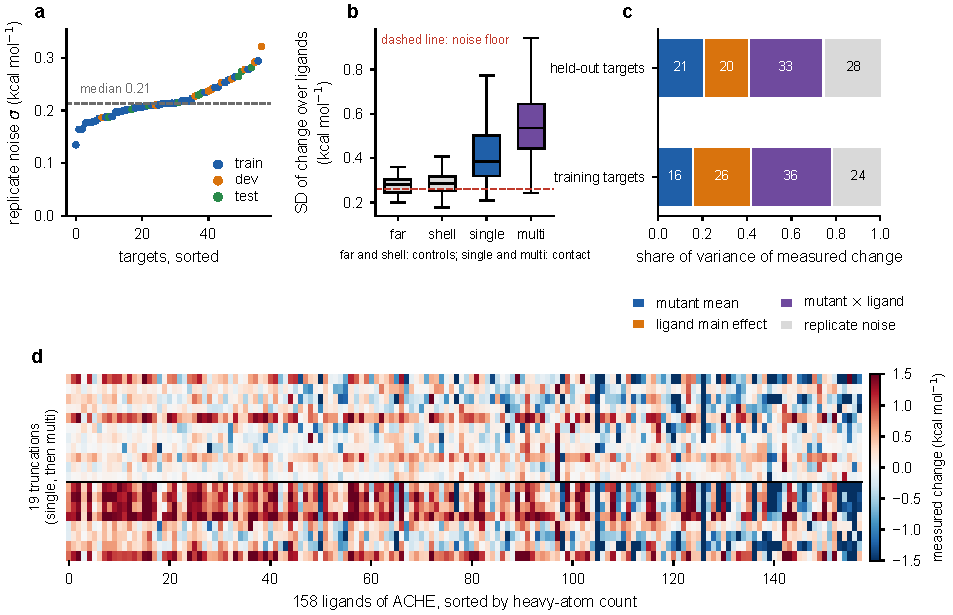
\includegraphics[width=\linewidth]{figures/fig2_response}
\caption{Response of the docking engine to receptor truncations. (a) Replicate noise of the wild-type score for each target. (b) Standard deviation over ligands of the measured change for shell and far controls, single contact truncations and multi-residue truncations; the dashed line marks the median noise of a change (\dsigmaMed{}~\kcal{}). (c) Share of the variance of measured changes held by the mean change of an edit, a ligand main effect, the edit-by-ligand interaction and replicate noise. (d) Measured changes for one held-out target (acetylcholinesterase): rows are truncations (single above the line, multi-residue below), columns are ligands ordered by heavy-atom count.}
\label{fig:response}
\end{figure}

The measured changes have a regular structure (Figure~\ref{fig:response}c,d). Replicate noise accounts for \shareNoise{}\% of their variance, the mean change of an edit for \shareMutant{}\%, a ligand main effect shared by all edits of a target for \shareLigand{}\% and the edit-by-ligand interaction for \shareInter{}\%. The ligand main effect follows a size law: in \nNegSlope{} of \nSlopeTargets{} targets, larger ligands gain more from a truncation than smaller ones. Figure~\ref{fig:response}d shows the pattern for acetylcholinesterase, where multi-residue truncations worsen the scores of small ligands and improve those of large ligands. The slope of this size dependence ranges from \slopeMin{} to \slopeMax{}~\kcal{} per heavy atom and is steeper in buried pockets ($r$ = \rBuried{} with the buried fraction of free space and \rAtomsTen{} with the number of receptor atoms within 10~\AA{} of the box center). Part of the interaction term follows the pose. For single contact truncations, the mean absolute change of a ligand rises from \contactNone{}~\kcal{} when no atom of its wild-type pose lies within 4.5~\AA{} of the removed side chain to \contactMany{}~\kcal{} when six or more atoms do, a trend present in \nContactTargets{} of \nContactOf{} targets, and the number of contacts correlates with the size of the change at $r$ = \rPoseContact{}. Controls without contact change by \controlNoContact{}~\kcal{}.

\subsection{Baseline surrogates do not respond to pocket edits}

We asked the baseline surrogates to predict the same changes for the \nHeldTargets{} held-out targets. Each model received the graph of the edited pocket, and its predicted change is the score for the edited pocket minus the score for the wild-type pocket. The three seed ensembles of the baselines respond with standard deviations of \sdPredRefMin{} to \sdPredRefMax{}~\kcal{} and the nine single checkpoints with \sdCkptMin{} to \sdCkptMax{}~\kcal{}, which is \ratioSdRefMin{} to \ratioSdRefMax{} times (single checkpoints \ratioCkptMin{} to \ratioCkptMax{} times) smaller than the \sdTrue{}~\kcal{} of the measured changes (Figure~\ref{fig:main}a). The correlation with the measured changes over all contact edits is \rRefSeedMin{} to \rRefSeedMax{} for single seeds. The seed ensembles reach \rEnsCZero{} (95\% interval \rLoCZero{} to \rHiCZero{}), \rEnsCOne{} (\rLoCOne{} to \rHiCOne{}) and \rEnsCTwo{} (\rLoCTwo{} to \rHiCTwo{}) for the plain, the within-target ranking and the cross-target ranking objective, and they separate contact edits from shell and far controls with AUCs of \aucRefMin{} to \aucRefMax{}. The hit-probability head of the baselines, which ranked ligands in the preceding analysis, gives the same picture with seed ensembles of \rEnsCZeroL{}, \rEnsCOneL{} and \rEnsCTwoL{} for its minus logit (Table~\ref{tab:main}).

\siinputpatched{table2}{Table S7}{Table~\ref{tab:si_levels}}

\subsection{Pocket geometry gives a surrogate its first response to edits}

The residue-sum network without geometry is as blind as the baselines when it is trained on wild-type scores only (pooled $r$ = \rEnsRsWt{}, 95\% interval \rLoRsWt{} to \rHiRsWt{}). Ten geometric descriptors of the pocket in its global term change this. The geometry network trained on wild-type scores alone has never seen an edited receptor, and it predicts the measured changes with $r$ = \rEnsRsgWt{} (\rLoRsgWt{} to \rHiRsgWt{}; \nSeedRsgWt{} seeds). The wild-type data already contain a relation that can produce this response: the score of a ligand depends on the size of the cavity, the descriptors expose that size to the network, and removing a side chain moves the prediction along the learned relation.

The response does not come from the residue graph. Removing the residue terms at inference, so that the score keeps only the ligand term and the global descriptor term, leaves the pooled correlation of the seed ensemble at \ablNoResRsgWt{} for the geometry networks trained on wild-type scores (full model \ablFullRsgWt{}), \ablNoResRsgInt{} for the geometry networks trained on measured changes (\ablFullRsgInt{}) and \ablNoResRsghInt{} for the networks with a hit head (\ablFullRsghInt{}). The predicted change of these networks is a function of the ligand embedding and the ten descriptors, and the residue graph adds no measurable response.

Interventional training raises the pooled correlation for the geometry-free residue-sum network, which goes from \rEnsRsWt{} to \rEnsRsInt{} (difference \diffRsIntMinusRsWt{}, 95\% interval \diffLoRsIntMinusRsWt{} to \diffHiRsIntMinusRsWt{}), and for the network that also receives an edit record, which goes from \rEnsRseWt{} to \rEnsRseInt{} (difference \diffRseIntMinusRseWt{}, interval \diffLoRseIntMinusRseWt{} to \diffHiRseIntMinusRseWt{}) (Figure~\ref{fig:main}e, Table~\ref{tab:main}); no label-shuffled control was trained for the geometry-free architecture. The increase is unresolved for the geometry network (\rEnsRsgWt{} to \rEnsRsgInt{}, difference \diffRsgIntMinusRsgWt{}, interval \diffLoRsgIntMinusRsgWt{} to \diffHiRsgIntMinusRsgWt{}) and for the dual encoder (\rEnsBfiveWt{} to \rEnsBfiveInt{}). The measured changes thus give a geometry-free network a response that a geometry network obtains from wild-type data, and they add a smaller increment on top of geometry. The edit-record network has the highest neural correlation (\rEnsRseInt{}), and the geometry network selected by the registered rule reaches \rEnsRsgInt{}; the two differ by \diffRsgIntMinusRseInt{} (\diffLoRsgIntMinusRseInt{} to \diffHiRsgIntMinusRseInt{}). All networks stay far below the noise ceiling of \ceilingR{} that follows from the wild-type replicates.

The hit head leaves this response intact (Table~\ref{tab:si_hyper} and Table~\ref{tab:main}). The network with a hit head, trained with three seeds and without label controls, reaches $r$ = \rEnsRsghWt{} without edited receptors and \rEnsRsghInt{} (\rLoRsghInt{} to \rHiRsghInt{}) with interventional training, for the seed ensemble (single seeds \rSeedMinRsghInt{} to \rSeedMaxRsghInt{}). This is \diffRsghIntMinusRsgInt{} above the six-seed registered geometry network (interval \diffLoRsghIntMinusRsgInt{} to \diffHiRsghIntMinusRsgInt{}) and \diffRsghIntMinusRsghWt{} above its wild-type-only version (\diffLoRsghIntMinusRsghWt{} to \diffHiRsghIntMinusRsghWt{}). It differs from the boosting model with pocket geometry by \diffRsghIntMinusGbmGeo{} (\diffLoRsghIntMinusGbmGeo{} to \diffHiRsghIntMinusGbmGeo{}).

\subsection{Label controls and descriptor models show what the response contains}

The analysis plan named two conditions for a claim that training on measured changes teaches a network to read the pocket: a pooled $r$ above the descriptor models and above both controls with permuted labels, with intervals over targets that exclude the control values. Neither condition holds. The geometry network trained on measured changes reaches $r$ = \rEnsRsgInt{} (\rLoRsgInt{} to \rHiRsgInt{}) for the seed ensemble. A boosting model on ligand descriptors, edit descriptors and pocket geometry reaches \rEnsGbmGeo{} (\rLoGbmGeo{} to \rHiGbmGeo{}), which exceeds the network by \diffGbmGeoMinusRsgInt{} (\diffLoGbmGeoMinusRsgInt{} to \diffHiGbmGeoMinusRsgInt{}), and the same model without the pocket descriptors reaches \rEnsGbmDesc{}. Networks trained on labels that were permuted over ligands, over edits or over all pairs give \rEnsRsgShl{}, \rEnsRsgShm{} and \rEnsRsgSha{}. The first implementation of the last two drew uniform permutations, which leave the row of an edit in place with probability one in six, so that these controls kept a fraction of the edit-specific signal. We corrected this after the held-out results were known and trained derangements instead, which give \rEnsRsgShmTwo{} and \rEnsRsgShaTwo{}. The corrected controls do not fall below the networks trained on measured labels: the difference in $r$ (measured labels minus control) is \diffRsgIntMinusRsgShmTwo{} (interval \diffLoRsgIntMinusRsgShmTwo{} to \diffHiRsgIntMinusRsgShmTwo{}) for the derangement over edits and \diffRsgIntMinusRsgShaTwo{} (\diffLoRsgIntMinusRsgShaTwo{} to \diffHiRsgIntMinusRsgShaTwo{}) for the derangement of all labels.

Pooled $r$ mixes differences between targets, between the edits of one target and between ligands. Separating these levels shows where the response sits (Figure~\ref{fig:levels}a--c). Within a target, the geometry network trained on measured changes reaches $r$ = \lvTargetRsgInt{}, the corrected controls \lvTargetRsgShmTwo{} and \lvTargetRsgShaTwo{}, and the boosting model with geometry \lvTargetGbmGeo{}. The edit means of a target, which rank the truncations by how strongly they move the scores, are predicted with \lvEditRsgInt{} by the geometry network, \lvEditRsgShmTwo{} and \lvEditRsgShaTwo{} by the corrected controls, \lvEditRsgWt{} by the geometry network without edited receptors and \lvEditGbmGeo{} by the boosting model. The ligand-specific part, the variation between ligands for one edit, stays at \lvLigRsgInt{} for the geometry network and \lvLigGbmGeo{} for the boosting model, and it reaches \lvLigGbmPoseGeo{} when the boosting model also receives the number of ligand atoms that touch the removed side chain in the wild-type pose. The ceiling for this level is \ceilLig{}. The ligand-specific part combines the ligand main effect and the edit-by-ligand interaction, and every model leaves most of it unexplained (Table~\ref{tab:si_levels}).

\begin{figure}[!ht]
\centering
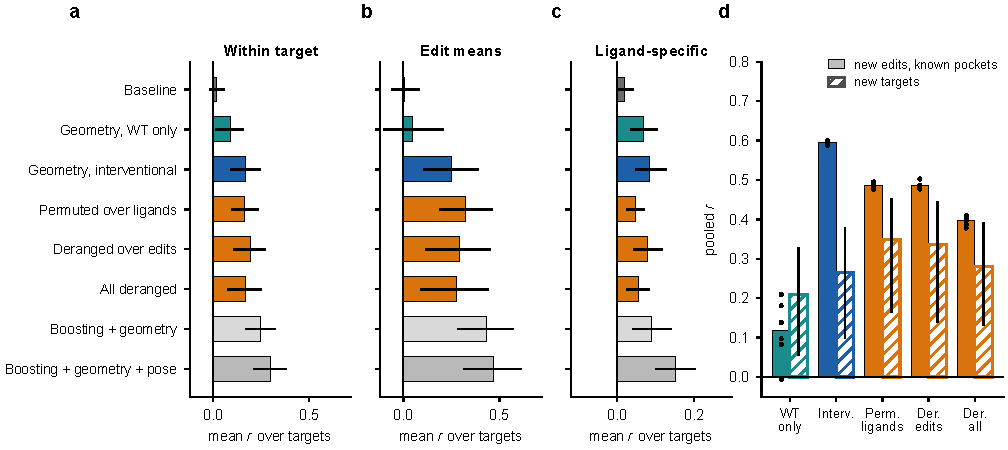
\includegraphics[width=\linewidth]{figures/fig4_levels}
\caption{Where the response comes from. Mean over the 19 held-out targets of (a) the correlation within a target over all contact pairs, (b) the correlation of the edit means within a target and (c) the ligand-specific correlation within an edit, with 95\% intervals over targets. (d) Pooled correlation for new edits of the training targets (15\% of their truncated receptors, withheld from training; solid bars with seeds as dots) and for new targets (hatched bars, seed ensemble with 95\% interval).}
\label{fig:levels}
\end{figure}

Measured labels make a difference where the network has seen the pocket or its relatives (Figure~\ref{fig:levels}d). For the 15\% of truncated receptors of each training target that were withheld from training (\shareMultiTrain{}\% of the contact edits among them are multi-residue truncations), the geometry network trained on measured changes reaches $r$ = \knownRRsgInt{} (SD over \nSeedRsgInt{} seeds \knownRSdRsgInt{}). Networks trained on deranged labels reach \knownRRsgShmTwo{} and \knownRRsgShaTwo{}, the control that permutes labels over ligands \knownRRsgShl{}, and the geometry network without edited receptors \knownRRsgWt{}. Measured labels thus carry edit-specific knowledge worth 0.1 to 0.2 in $r$ for a pocket the network has seen, and the controls show that the remaining 0.4 to 0.5 comes from what any label set of a target contains, namely the scale of its responses and its ligand main effect. For a target of an unseen family the edit-specific knowledge brings no measurable gain in any of the three levels (Figure~\ref{fig:main}e and Figures~\ref{fig:levels}a--c).

\subsection{The response to edits grows with the number of edits and transfers within a family}

The response to edits in new targets rises with the number of edits per training target (Figure~\ref{fig:scale}b). Pooled $r$ on the held-out targets is \scaleRMkTwo{} with 2 edits kept per training target, \scaleRMkEight{} with 8, \scaleRMkTwelve{} with 12 and \scaleRFull{} with all edits (on average \editsAllMean{}), and the 15\% withhold leaves \editsLeftTwo{}, \editsLeftEight{}, \editsLeftTwelve{} and \editsLeftFull{} edits for training. It also rises with the number of training targets, from \scaleRNtFour{} with 4 targets through \scaleRNtSixteen{} with 16 to \scaleRNtTwentyfour{} with 24 and \scaleRFull{} with all 38 (Figure~\ref{fig:scale}a). Each setting was trained with two seeds that differ by up to 0.29, so that the trends carry information and single points do not. The scaling runs have no label controls, and the network trained on wild-type scores alone reaches \rEnsRsgWt{} on the same targets, so the curves show how many edits and targets interventional training needs to reach that level.

\begin{figure}[!ht]
\centering
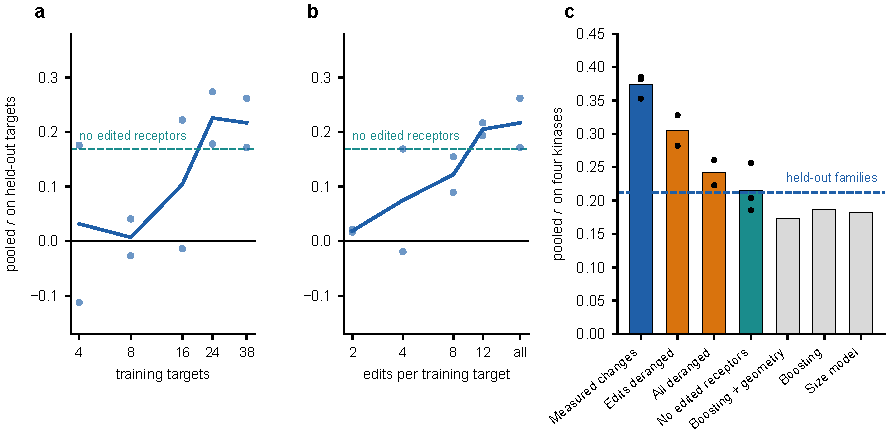
\includegraphics[width=\linewidth]{figures/fig5_scale}
\caption{The response to edits grows with the number of edits and transfers within a family. The scaling runs (a, b) have no label controls. Pooled correlation on the 19 held-out targets after training with (a) fewer training targets and (b) fewer edits per training target (dots: two seeds; line: mean; dashed line: geometry network without edited receptors, mean of six seeds). (c) Pooled correlation on four kinases withheld from training (ABL1, EGFR, SRC, JAK2) for the geometry network trained on measured changes, its controls and descriptor models fitted on the same training targets (dots: seeds; dashed line: the same network on the 19 held-out targets of other families).}
\label{fig:scale}
\end{figure}

Four kinases (ABL1, EGFR, SRC and JAK2) were withheld together with all their edits and the network was trained on the other 34 training targets, which include 17 further kinases (Figure~\ref{fig:scale}c). The geometry network trained on measured changes predicts the withheld kinases with $r$ = \kinRRsgInt{} (\kinNRsgInt{} seeds), against \kinRRsgWt{} for the network without edited receptors, \kinRRsgShmTwo{} and \kinRRsgShaTwo{} for deranged labels (\kinNRsgShmTwo{} seeds each) and \kinRGbmGeo{} for the boosting model with geometry. The edit means of the withheld kinases are predicted with \kinEditRsgInt{} by the network trained on measured changes and with \kinEditRsgShmTwo{} and \kinEditRsgShaTwo{} by the controls. The result covers four targets and has no interval over targets. The network trained on measured changes exceeds the controls with deranged labels by \kinGapRsgShmTwo{} and \kinGapRsgShaTwo{} in pooled $r$.

\subsection{The cached state evaluates edited pockets in a virtual alanine scan}

The same state evaluates an edited pocket by re-encoding it. We used this to truncate every residue with a side chain within 14~\AA{} of the box center of one held-out target, which was fixed before the scan as the target with the median per-target correlation (DHFR, \scanEdits{} residues), and to predict the change of the score of all \scanLig{} ligands (Figure~\ref{fig:scan}). The \scanModels{} seeds evaluated \scanPairs{} million ligand-edit pairs in \scanAllSec{} s, of which \scanQuerySec{} s were queries and the rest featurization and the construction of the edited graphs, against \dockDays{} GPU-days of docking, about \speedup{} times the time of the scan.

\begin{figure}[!ht]
\centering
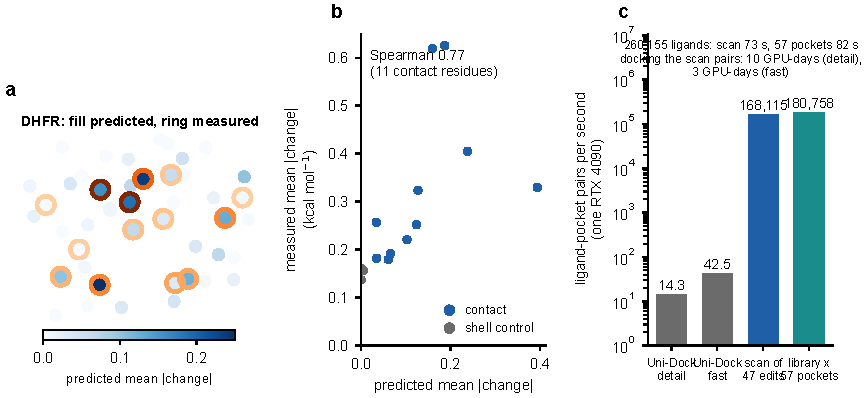
\includegraphics[width=\linewidth]{figures/fig7_scan}
\caption{Throughput of the cached pocket state and virtual alanine scan of a held-out target (DHFR, the target with the median per-target correlation). (a) C$\alpha$ positions of the 47 scanned residues projected on the plane of largest spread, filled by the predicted mean absolute change of the truncation over 260,155 ligands (three-seed ensemble of the geometry network) and ringed by the measured mean absolute change over 160 ligands for the 14 docked residues. (b) Predicted against measured mean absolute change of the docked residues. (c) Ligand-pocket pairs per second of GPU docking (Uni-Dock, detail and fast mode at the batch size with the highest rate), of the virtual scan of 47 edits and of the screen of the library against 57 wild-type pockets, on one RTX 4090 (ensemble of the three registered geometry networks without hit head, including ligand featurization and, for the scan, the construction of the edited graphs).}
\label{fig:scan}
\end{figure}

The predicted map agrees with the measured one in magnitude and differs in sign. Across the \scanNContact{} contact residues of DHFR with measured changes, the predicted mean absolute change has a Spearman correlation of \scanSpearmanAbs{} with the measured one (\scanSpearmanAbsAll{} with the three shell controls included), while the predicted mean signed change has $r$ = \scanRSigned{} with the measured one. Over all held-out targets the ranking of single contact truncations by predicted mean absolute change has a mean Spearman correlation of \hotRsgInt{} with the measured ranking, against \hotDist{} for the distance of the residue to the box center alone. The scan ranks the single contact truncations of a target below the distance of the residue to the box center (mean Spearman correlation \hotRsgInt{} against \hotDist{}), and its ligand-specific predictions correlate with the measured ones at \lvLigRsgInt{} against a ceiling of \ceilLig{} (Figure~\ref{fig:levels}c).
